\section{Royale with Cheese}
Recall Burgers equation from Example 1.5 of the lecture script :
\begin{align*}
	\dot{u} + u \partial_x u = 0
	.\end{align*}
Note this is a scalar conservation law :
\begin{align*}
	\dot{u} + f'(u) \partial_x u = 0
	.\end{align*}
Burgers equation arises by $f = \frac{1}{2} u^2$
\begin{question}
	According to Theorem 1.4 there is a unique $\mathcal{C}^{1} $ solution to this IVP at least when t is small.
	For how long does the theorem guarantee that the solution exists uniquely
\end{question}
\begin{solution}
	Theorem 1.4 gives us a condition for the domain on which a unique solution exists based on if the characteristics cross or not,
	it does so by considering the characteristic equation of Burgers equation, we see that :
	\begin{align*}
		z(s) = u(x(s),t(s)) \implies  z'(s) = \partial_x u x' + \dot{u} t'
		.\end{align*}
	Which means we should choose $x' = u$ and $t' = 1 $ this leads us to :
	\begin{align*}
		x(s) & = u*s + x_{0} \\
		t(s) & = s+t_{0}
		.\end{align*}
	and :
	\begin{align*}
		z'(s) = 0
		.\end{align*}
	Such that $z$ is constant i.e the value of $u(x(s),s)$ is constant on one characteristic.
	We can determine this value by using the initial condition :
	% \begin{align*}
	% 	z(0) = u(x(0),t(0)) = u(x_{0},t_{0}) \myS{t_{0}=0}{=} u(x_{0},0) = g(x_{0})
	% .\end{align*}
	Such that $x(s) = s*g(x_{0}) + x_{0}$ or with arbitrary f $x(s) = s*f'(g(x))+x$, for there to be a unique solution the characteristics can not cross
	for this we want $x \mapsto x+s*f'(g(x))$ to be monotone increasing i.e it is bijective :
	\begin{align*}
		1+s*f^{''}(g(x))g'(x) > 0  \ \leftrightarrow \ 1-t\alpha >0
		.\end{align*}
	which leads to the condition that we get a unique solution for $t< \frac{1}{\alpha } $ \\[1ex]
	In our case we have :
	\begin{align*}
		f'' & = 1  \\
		g'  & =  1 \\
		.\end{align*}
	Such that $f^{''}(g(x))g' > 0 (= \alpha )$  and we get a unique solution on $\mathbb{R} \times  [0,\infty)$
\end{solution}
\begin{question}
	Derive the characteristic equations
\end{question}
\begin{solution}
	As we ve seen above :
	\begin{align*}
		z(s) = u(x(s),t(s)) \implies  z'(s) = \partial_x u x' + \dot{u} t'
		.\end{align*}
	Which means we should choose $x' = u$ and $t' = 1 $ this leads us to :
	\begin{align*}
		x(s) & = u*s + x_{0} \\
		t(s) & = s+t_{0}
		.\end{align*}
	With $z' = 0$ implying :
	\begin{align*}
		x(s) & = x*s+x \\
		t(s) & = s     \\
		.\end{align*}
\end{solution}
\begin{question}
	On a $(x,t)-$plane draw the characteristics and describe the behaviour of this solution
\end{question}
\begin{solution}
	We need to draw :
	\begin{align*}
		x = x_{0}*t + x_{0}
		.\end{align*}
    On a $(x,t)$ plane : 
    \begin{align*}
      t = \frac{x-x_{0}}{x_{0}}
    .\end{align*}
    To avoid division by zero :
    \begin{align*}
      t = \frac{x-x_{0}}{x_{0}+\epsilon }
    .\end{align*}
    \begin{figure}[H]
     \centering 
     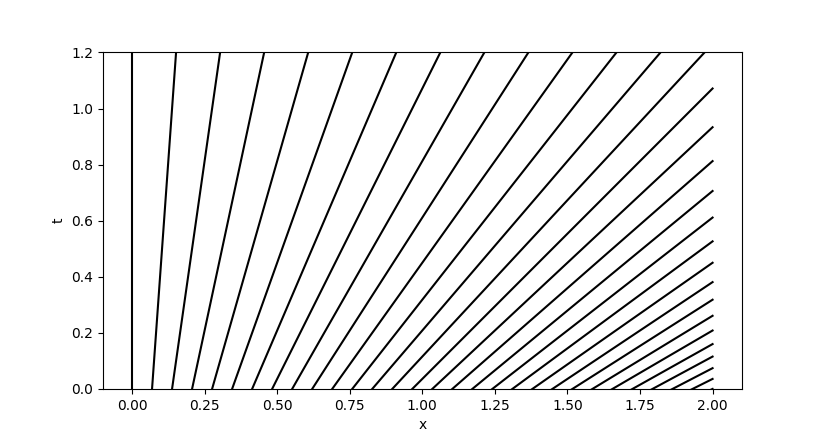
\includegraphics[scale=0.5]{figures/sheet_3_burger.png} 
   \end{figure}
\end{solution}
\begin{question}
 Derive the solution to the IVP 
\end{question}
\begin{solution}
  To recap what we know : 
  \begin{align*}
		x(s) & = x_{0}*s+x_{0} \\
		t(s) & = s     \\ 
    z(s) &= u(x_{0}*s+x_{0},s) = g(x_{0})
  .\end{align*}
No for arbitrary $(x,t) \in \mathbb{R}\times \mathbb{R}$ determine the characteristic :
\begin{align*}
  x &= x_{0}+t +x_{0} \\
.\end{align*}
this implies 
\begin{align*}
 x = x_{0}*(1+t) \implies x_{0} = \frac{x}{1+t}
.\end{align*}
Which means  
\begin{align*}
  u(x,t) = g(\frac{x}{1+t} = \frac{x}{1+t}
.\end{align*}
\end{solution}
\begin{question}
 Verify this is indeed a solution  
\end{question}
\begin{solution}
 We check $u(x,0) = \frac{x}{1+0} = x = g(x)$  and : 
 \begin{align*}
   \dot{u} + u \partial_x u =  - \frac{x}{(1+t)^2}  + \frac{x}{1+t}*\frac{1}{1+t}  = 0
 .\end{align*}
\end{solution}
\begin{question}
 Explain why the method of characteristics is well-suited to solving first order PDEs that are linear in the derivatives 
\end{question}
\begin{solution}
  We can use the chain rule to reduce the problem to a system of ODEs
\end{solution}
\section{Solving PDEs}



